\documentclass{article}
%\usepackage{fancyhdr}
\usepackage{epstopdf}
\epstopdfsetup{update}
% Language setting
% Replace `english' with e.g. `spanish' to change the document language
\usepackage[english]{babel}
\usepackage{/usr/share/texlive/texmf-dist/tex/generic/nopageno/nopageno}
% Set page size and margins
% Replace `letterpaper' with`a4paper' for UK/EU standard size
\usepackage[letterpaper,top=2cm,bottom=2cm,left=3cm,right=3cm,marginparwidth=1.75cm]{geometry}

% Useful packages
\usepackage{amsmath}
\usepackage{graphicx}
\usepackage[colorlinks=true, allcolors=blue]{hyperref}

\title{Summary of Aortic Root Analysis}
\author{Ankush Aggarwal\thanks{A. Aggarwal is with the
Glasgow Computational Engineering Centre, James Watt School of Engineering, University of Glasgow, Glasgow, UK (e-mail:ankush.aggarwal@glasgow.ac.uk). }, Peter Mortensen, Jilei Hao, Lukasz Kaczmarczyk, \\ 
Albert T. Cheung, Lourdes Al Ghofaily, Robert C. Gorman, \\Nimesh D. Desai, Joseph E. Bavaria, Alison M. Pouch \thanks{A. Pouch is with the Departments of Radiology and Bioengineering, University of Pennsylvania, Philadelphia, PA, USA (e-mail: pouch@pennmedicine.upenn.edu).}
%
\thanks{This work was supported in part by the Chan Zuckerberg Initiative 2020-219012 grant, the Institute of Physics and Engineering in Medicine, and the National Heart Lung and Blood Institute (K01-HL141643).}
}

\begin{document}
\maketitle
\begin{figure}[h!]

\includegraphics[width = 0.25\linewidth]{UPennLogo}~~~~~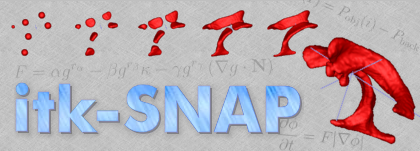
\includegraphics[width = 0.25\linewidth]{ITKSnapLogo}~~~~~
\includegraphics[width = 0.25\linewidth]{GlaLogo}~~~~~
\includegraphics[width = 0.1\linewidth]{GCEC}
\end{figure}
\newpage
\subsection*{Visualisation Toolkit polydata or vtp files}
For each frame submitted, there is now a .vtp file which includes the new biomedical values that have been calculated. This data is best viewed in the free software, paraview. 

The data now included are either specific to the points, to the cells, or are are uniform over the whole field.
The point specific values are:
\\
The root anatomy - 
\begin{itemize}
    \item STJ - Marks the sinotubular junction with value 1 and 0 elsewhere.
    \item VAJ - Marks the ventriculo-aortic junction with value 1 and 0 elsewhere.
    \item IAS - Marks the interatrial septum with value 1 and 0 elsewhere.
    \item Label - ???
\end{itemize}
The root properties - 
\begin{itemize}
    \item Curv$\_$Gaussian - The gaussian curvature, at each point.
    \item Curv$\_$Mean - The mean curvature, at each point.
    \item J$\_$Pt - The jacobian, at each point.
    \item I1$\_$Pt - The principle strain, at each point.
    \item Motion - The motion of each point between the time frames.
    \item Total$\_$Motion - The cumulative motion, at each point. 
    \item Thickness - The wall thickness of the root, at each point.
    \item Radius - The distance from the wall centre to the wall edge, at each point.
    \item Circ$\_$Strain$\_$Pt - the Circumferential strain, at each point.
    \item Long$\_$Strain$\_$Pt - the Longitudinal strain, at each point.
\end{itemize}
Vectors - 
\begin{itemize}
    \item - Circumferential - The circumferential vector of the node.
    \item - Longitudinal - The logitudinal vector of the node.
    \item - Normal - The normal vector of the node.
    \item - Displacement$\_$Wall - The displacement of the root wall, relative to the root centre, at each point.
    \item - Displacement$\_$Root - The displacement of root, without the wall movement at each point.
    \item - Displacement$\_$Total - The displacement of each point, with both the wall and root displacements.
\end{itemize}
The cell specific values:
\begin{itemize}
    \item J - The jacobian, at each cell.
    \item I1 - The principle strain, at each cell.
    \item Circ$\_$Strain - the Circumferential strain, at each cell.
    \item Long$\_$Strain - the Longitudinal strain, at each cell.
\end{itemize}
The field values:
\begin{itemize}
    \item WallArea - The total wall area of the frame.
    \item WallVolume - The total wall volume of the frame.
    \item LumenVolume - The total lumen volume of the frame.
    \item ValvePosition - A label specifiying if the valve is open (value of 1) or closed (value of 0).
\end{itemize}
\subsubsection*{Visualisation}
When all the frames are loaded in paraview the frames can be cycled through. The movements of the root have been separated so that the wall movement, without the movement of the whole root, and the root movement, without the wall movement, can be viewed separately. The default has the movement fixed to the position of the reference frame. To view the movements, apply the 'Warp By Vector' filter and chose the relevant displacement vector (wall, root or total displacement).

The point vectors can be visualised with the filter 'Glyphs'.

\subsubsection*{CSV data files}
Also included are two .csv files which contain average values and field values for each time frame. There is a raw data set, in which the time points are determined by the original frames submitted and the time between each. The second set has the the time standardised, so that different data sets can be more readily compared. It should be noted that, for the standardised time, it has been assumed that the cycle starts before when the valve opens and that the ratio of the valve being open to it being closed is 1:2.


\newpage
\subsection*{Global Result Figures}

\begin{figure}[h!]
\centering
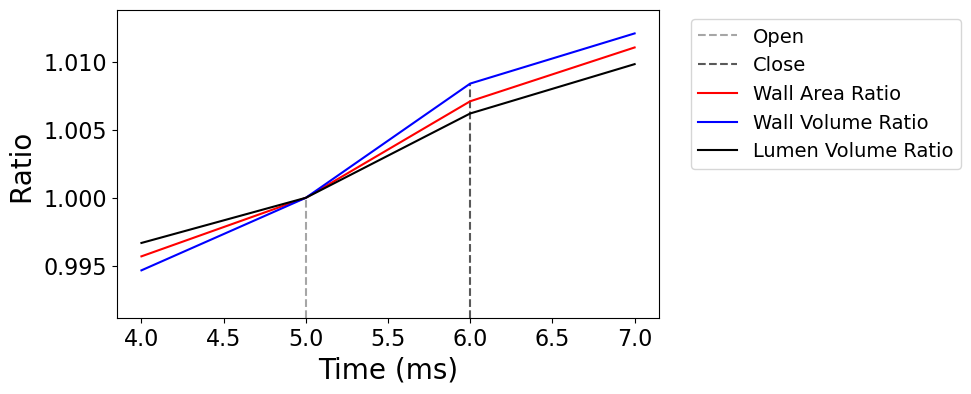
\includegraphics[width=0.75\textwidth]{NormalisedDataOriginalTime.png}
\caption{Wall area, wall volume and lumen volume ratio, with original time data.}
\end{figure}


\begin{figure}[h!]
\centering
\includegraphics[width=0.75\textwidth]{NormalisedDataStandardisedTime.png}
\caption{Wall area, wall volume and lumen volume ratio, with standardised time data.}
\end{figure}


\begin{figure}[h!]
\centering
\includegraphics[width=\textwidth]{RawDataOriginalTime.png}
\caption{Raw data of wall area, wall volume and lumen volumes, with original time data.}
\end{figure}

\begin{figure}[h!]
\centering
\includegraphics[width=\textwidth]{RawDataStandardisedTime.png}
\caption{Raw data of wall area, wall volume and lumen volume ratio, with standardised time data.}
\end{figure}

\end{document}
